\section{Toy Models}

\subsection{Model Properties and Simulation Methods}

The dynamics of the transitions between two square boxes in a simple two-dimensional periodic potential of the form

\begin{equation}
\label{eq:toy-pel}
\mathscr{V}(x,y) = \cos (2 \pi x) + \cos (2 \pi y) 
\end{equation}
were examined.
Such a potential has many periodic orbits and the motion in $x$ is completely independent of the motion in the $y$ direction and {\it vice versa}.
Therefore, a randomisation potential was introduced by adding randomisation lines.
If such a line is crossed, the direction of the velocity vector is rotated by an angle uniformly distributed between 0 and $2 \pi$.
The line can be physically interpreted as an infinitely thin wall of alternating charges, which changes the direction of a passing charged particle.
Box A is defined as the region $-1 < x < 0$ and $ 0 < y < 1$.
Box B is defined by $0 < x < 1$ and $ 0 < y < 1$.
The boundary conditions can be viewed as a simulation on the surface of a torus.
A particle exiting box A or B through the line $y = 1$ simply enters the same box from the line $y = 0$, while its velocity remains unchanged.
The boxes have two boundaries, $x = 1$ (which is in an analogous way connected to $x = -1$) and $x = 0$.
The randomisation lines were folded to 5 overlapping circles with radii of 0.2 located at [0.3,0.3], [0.3,0.7], [0.5,0.5], [0.7,0.3] and [0.7,0.7] in box B and at the equivalent positions in box A.

\begin{figure}[h]
\centering
\psfrag{time}{time}
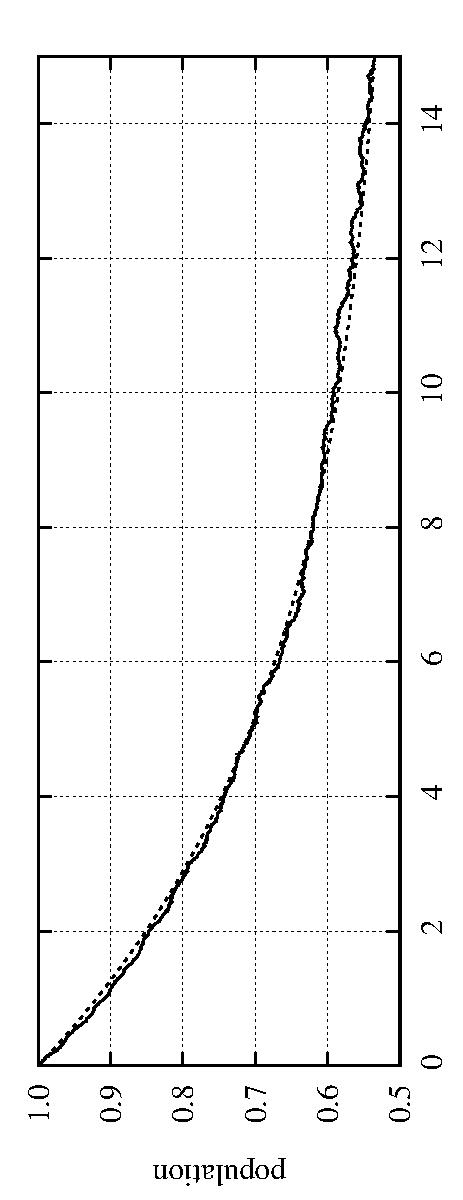
\includegraphics[height=14cm, angle=270]{Images/me-exp.pdf}
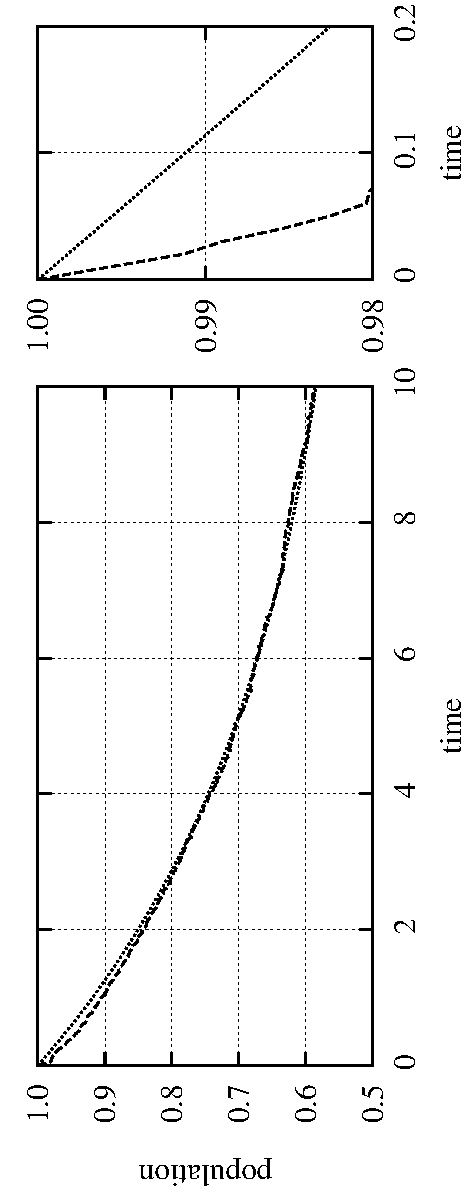
\includegraphics[height=14cm, angle=270]{Images/merough-exp.pdf}
\caption[Exponential kinetics of the toy models.]{Evolutions of the populations obtained from the ME simulations for the smooth (top) and the rough (bottom left) dividing surfaces. The dashed (top) and dotted (bottom) lines were obtained by fitting the ME evolutions to an exponential function. A steep decay corresponding to recrossing can be found for the rough dividing surface at small time values (bottom right). Nevertheless, ME dynamics of the used toy models are exponential even for high energies ($E$=0.5). The models are suitable for description in terms of the master equation.}
\label{fig:me-exp}
\end{figure}

Classical microcanonical simulations using the velocity Verlet integrator\cite{Verlet1967} with time step d$\tau$=0.01 were used both for BXD and ME simulations.
The ME simulation here stands for a direct simulation of relaxation of the population of $10^3$ independent particles in box A from the state in which population in A equals $10^3$ and in B equals 0.
In both BXD and ME simulations, the particles were first equilibrated in a system comprising both boxes for $10^4$ steps.
In ME simulations of the ${\rm A \rightarrow B}$ transition process, all particles in B were deleted and the system was propagated for another $5\cdot10^4$ steps.
The concentration defined as the number of particles in box A divided by the number of particles in both boxes was recorded in each step.
The evolution was fitted to an exponential function (\ref{eq:A-to-B-and-back-a-of-t}).
As seen in figure \ref{fig:me-exp}, the ME dynamics for the system are exponential even for the rough dividing surfaces [$x = 0.05 \sin (20 \pi y)$ and $x = 1 + 0.05 \sin (20 \pi y)$].
BXD simulations were equilibrated in the same way.
Then, the simulations were constrained in the desired boxes for another $5\cdot10^4$ steps.
A particle hitting the dividing surface, for example in case of the smooth surface $x = -1$ or $x = 0$ for box A and $x = 0$ or $x = 1$ for box B, was returned to its previous position and the velocity direction was randomised, requiring only that the sign of its $x$ component pointed into the box.
The statistical error of each calculated rate constant was estimated as the standard deviation of values obtained from 15 independent simulations.
The simulation protocols were implemented and vectorised in Octave 3.2.\cite{Octave2012}

The microcanonical TST rate constant was calculated using the RRKM formula (\ref{eq:rrkm}).
Densities of states of both the dividing surface and the box were calculated numerically and fitted to a polynomial expansion.
Each configuration space box was discretised into a square grid of $10^6$ equally distant points, and the density of states was calculated for each one for energies between $-2$ and $2$.
The integral density of states $g(E)$ was then fitted with a linear function.
The function
\begin{equation}
\label{eq:rrkm-fit-gE}
g(E) = 3.653 + 4.321 E
\end{equation}
describes the exact $g(E)$ very well for energies between 0 and 0.5.
Both the smooth and the rough surfaces were discretised into grids of points with the distances between the neighbouring points set to $10^{-4}$.
The smooth surface can be well described with the function
\begin{equation}
\label{eq:rrkm-smooth-gE}
g^{\ddagger}(E) = 0.177 E
\end{equation}
for energy values between 0 and 0.5.
The integral density of states for the rough surface can be approximated with a polynomial fit as
\begin{equation}
\label{eq:rrkm-rough-gE}
g^{\ddagger}(E) = 0.008 + 0.359 E + 0.013 E^2 ~.
\end{equation}
The rate constants were calculated as
\begin{equation}
\label{eq:rrkm-rrkm-num}
k^{TST}_{\rm A \rightarrow B} (E) = 2 \times 2 \pi \times \frac{g^{\ddagger}(E)}{\frac{\rm d}{{\rm d} E} g(E)} ~,
\end{equation}
where the first factor of 2 follows from presence of two dividing surfaces between the boxes.
The numerical result for the smooth surface agrees well with the RRKM rate constant in the harmonic approximation:
\begin{equation}
\label{eq:rrkm-ha}
k^{HA}_{\rm A \rightarrow B} (E) = \Xi \frac{\nu_{\rm A}^\eta}{\nu^{\ddagger (\eta-1)}} \left( \frac{E - V^{\ddagger}}{E - V_{\rm A}} \right)^{\eta - 1} ~,
\end{equation}
which can be calculated for the toy model used in this work as
\begin{equation}
\label{eq:rrkm-ha-2}
k^{HA}_{\rm A \rightarrow B} (E) =  \frac{2 E}{E + 2} ~.
\end{equation}
Here $\Xi = 1$ is a degeneracy factor for the reaction, $\eta = 2$ is the number of degrees of freedom, $\nu_{\rm A} = 1$ is the harmonic vibrational frequency in the minimum of box A with energy $V_{\rm A} = -2$, and $\nu^{\ddagger} = 1$ at the harmonic frequency in the lowest energy point of the transition state ensemble, with energy $V^{\ddagger} = 0$. The factor 2 in (\ref{eq:rrkm-ha-2}) follows from the presence of two dividing surfaces ($x = 0$ and $x = -1$).


\subsection{Comparison of the TST and MFPT Approaches}

\begin{figure}[h!]
\centering
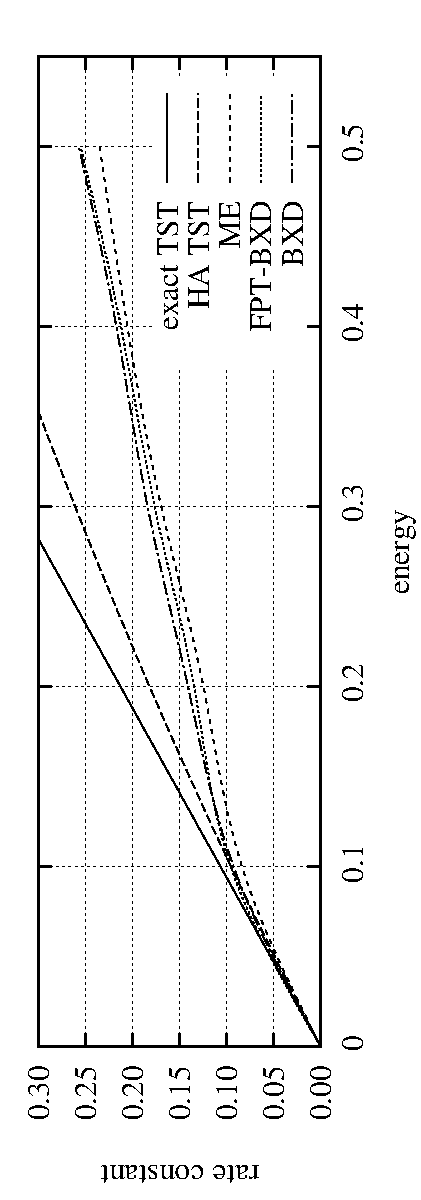
\includegraphics[height=15cm, angle=270]{Images/smooth.pdf}
\caption[Comparison of TST, harmonic TST, ME, BXD and FPT-BXD rate constants.]{Comparison of ME (the lowest dashed curve) rate constants for the smooth dividing surface with the rate constants from BXD simulations using the reactive flux (BXD) and the MFPT (FPT-BXD) formulation and with the exact RRKM (exact TST) and RRKM in the harmonic approximation (HA TST).}
\label{fig:tst-bxd}
\end{figure}

The results for ME and BXD simulations were calculated for energy values 0, 0.1, 0.2, 0.3, 0.4 and 0.5. 
Since the statistical errors are very small ($\Delta k_{\rm A \rightarrow B} < 0.005$), the curves can be fitted with cubic splines (figure \ref{fig:tst-bxd}). 
The rate constants calculated using the old and the new formulations of BXD agree well with the reference ME data for the smooth dividing surface.
The TST rate constants significantly differ from the reference ME rate constants at higher energies, where crossing the barrier is not the rate limiting process.
The rate constants all converge to 0 as $E \rightarrow 0$ and they seem to be consistent for low energies, $\lim_{E \rightarrow 0} k^i_{\rm A \rightarrow B} / k^j_{\rm A \rightarrow B} = 1$ (figure \ref{fig:tst-bxd}).
A dividing surface defined by the curve $x = 0.05 \sin (20 \pi y)$ (the total length of dividing surface $\approx 2.3 $ instead of 1 in the case of the smooth dividing surface) was used to demonstrate the large increase of the reactive flux rate constant with dividing surface roughness.
Comparison of the rate constants calculated using the new and the old BXD formulations and the ME demonstrates that the reactive flux approach significantly overestimates the rate constant if the dividing surface is rough (figure \ref{fig:mfpt-rough}).
The old formulation of BXD gives higher rate constants than the MFPT formulation.
The TST rate constant is non-zero for zero energy since the dividing surface contains points with $E<0$.

\begin{figure}[h!]
\centering
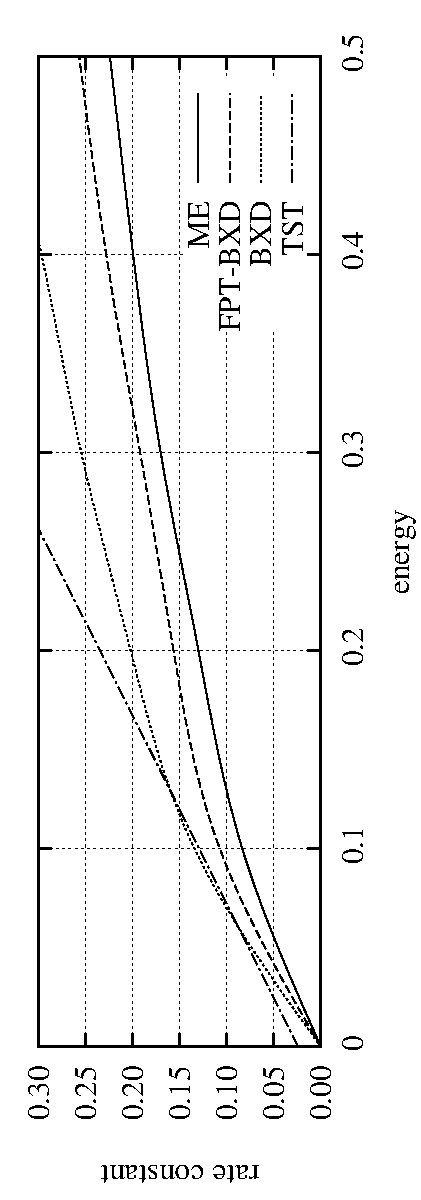
\includegraphics[height=15cm, angle=270]{Images/rough.pdf}
\caption[FPT-BXD results for a rough dividing surface.]{Dependence of the rate constants on energy for the rough dividing surface. The exact TST rate constant (dash-dot line) [see equation (\ref{eq:rrkm-rough-gE})] differs significantly from the reference ME (solid line) rate constant. The BXD rate constant based on the reactive flux formulation (dotted line) is generally higher than the FPT-BXD rate constant (dashed line). Since the statistical error is below 0.005, the data for $E$=0, 0.1, 0.2, 0.3, 0.4 and 0.5 were fitted with cubic splines. }
\label{fig:mfpt-rough}
\end{figure}

\subsection{Uneven Boxes}

An asymmetric term was added to study the effect of uneven equilibrium populations

\begin{equation}
\label{eq:toy-pel-uneven}
\mathscr{V}(x,y) = \cos (2 \pi x) + \cos (2 \pi y) + 0.2 \sin (\pi x) ~.
\end{equation}
The equilibrium constant and the reference rate constants were obtained by fitting the ME evolution.
Exit MFPT's for boxes were obtained from BXD simulations.
The rate constants calculated from exit MFPT's using equation (\ref{eq:corrected}) agree with the reference ME rate constants (figure \ref{fig:uneven}).


\begin{figure}[h!]
\centering
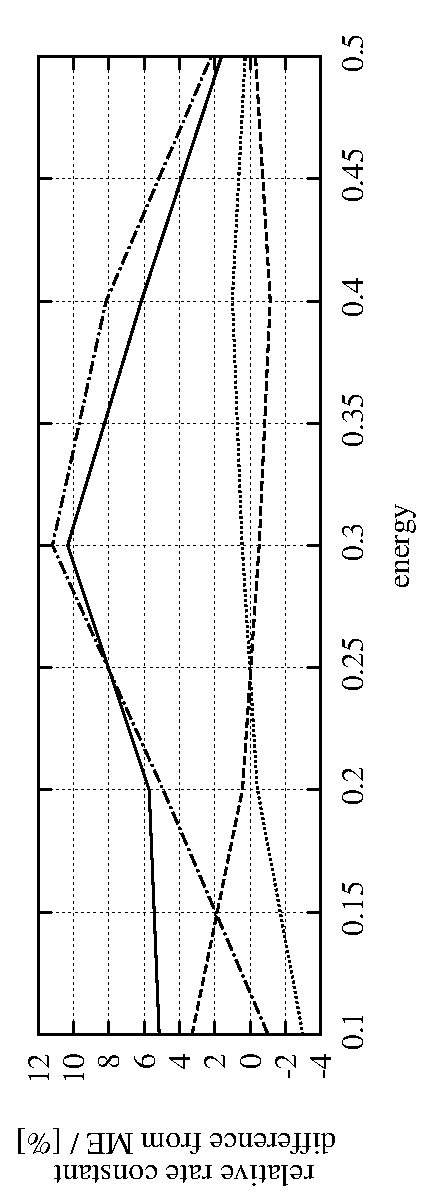
\includegraphics[height=15cm, angle=270]{Images/inequal.pdf}
\caption[FPT-BXD performance for uneven boxes.]{Comparison of rate constants obtained from FPT-BXD in boxes with potential (\ref{eq:toy-pel-uneven}). The relative difference in per cent is given as a function of energy. The statistical error of all values in the graph is roughly $\pm 3 \%$. Dashed and dotted lines represent the difference between ME rate constants (reference values) and FPT-BXD rate constants corrected with penetration times $k_{\rm A \rightarrow B}$ and $k_{\rm B \rightarrow A}$ using equation (\ref{eq:corrected}). The full and the dashed-dotted lines represent the difference between the ME rate constants and the exit FPT-BXD rate constants $k_{\rm A \rightarrow \partial AB}$ and $k_{\rm B \rightarrow \partial AB}$, respectively. The corrected FPT-BXD rate constants are in very good agreement with the reference ME values throughout the whole energy range.}
\label{fig:uneven}
\end{figure}

The projection of the density of states into configuration space (the probability distribution of coordinates) was studied for two constraining methods: bouncing from the wall according to Glowacki {\it et al.}\cite{Glowacki2009} and randomisation of the velocity direction.
As predicted in section \ref{sec:error}, the inversion procedure by Glowacki {\it et al.}\cite{Glowacki2009} artificially increases the population near box boundaries.
Randomisation of the velocity direction after hitting the boundary, requiring the $x$ component of velocity to point into the box, reproduces the correct distribution.

\subsection{Higher Dimensions}
\label{sec:manydim}

To demonstrate that the above derived results are transferable to PES's more relevant for molecular systems, a many-dimensional potential of the form

\begin{equation}
\label{eq:mendim}
\mathscr{V}({\bf p}) = \cos (2 \pi p_1) + \frac{1}{n} \sum_{i=1}^n a_n \sin (6 \pi {\bf p} \cdot {\bf c}_i) 
\end{equation}
was studied, where the parameters $a_i$ and ${\bf c}_i$ were selected as random numbers (uniform distribution) between 0 and 1.
In this work, an $n=7$-dimensional system was studied.
The box was defined as $p_i \in [0,1]$ for each $i$.
The potential has on average two minima in each dimension per box, so the total number of minima can be estimated as $2^7$.
Simulations show that such a potential does not need randomisation lines and the population evolution is roughly exponential.

Boxes defined by Voronoi tesselation for complex molecular systems can sometimes lack the funnel-like structure modelled in potential (\ref{eq:mendim}) with the first term.
Therefore, relaxation to equilibrium for the potential without the cosine term was also studied.
The evolution (figure \ref{fig:mendim-nocen}) can be decomposed into two exponentials.
A similar decomposition of species into more types was considered by Bunker and \mbox{Hase\cite{Bunker1964, Bunker1973, Hase1983}} for different potentials.
The decomposition might be used to describe systems divided into boxes with non-exponential kinetics more accurately in terms of the master equation.

\begin{figure}[h!]
\centering
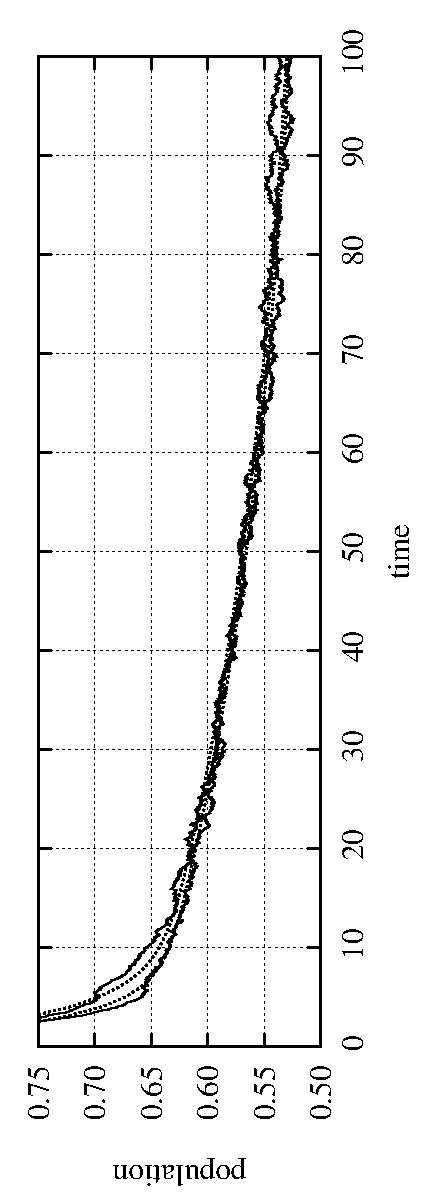
\includegraphics[height=15cm, angle=270]{Images/mendim.pdf}
\caption[Distribution of FPT for a box with many minima.]{Decomposition of FPT distributions of passing into two different neighbouring boxes. Potential (\ref{eq:mendim}) was used. For energy = 0.2, the weight of the slowly decreasing exponential is 0.32 for neighbour 1 and 0.31 for neighbour 2. The similarity of the weights suggests that the box can be subdivided into two phase space boxes.}
\label{fig:mendim-nocen}
\end{figure}


